% Generated from the matching Typst scaffold by
% scripts/migrate_typst_report_to_latex.py.

% ── 5.6  H5 and Task Interdependence: When Does Memory Matter? ────────────
% PURPOSE: Convert H5's near-null boundary into a mechanistic finding — memory matters
%          only on the interdependent fraction of tasks, and we can measure that fraction.
% MOVE: Counter-intuitive lead / convert near-null into mechanism — "not every task needs
%        memory", made measurable.
% FIGURES/TABLES: fig:memory-lift, fig:interdependence, tab:memory-lift.
% ─────────────────────────────────────────────────────────────────────────

\section{H5 and Task Interdependence: When Does Memory Matter?}
\label{sec:h5}

The headline result of this thesis is a powered null: on the resolution proxy no forgetting
policy differs from full-memory accumulation (Section~\ref{sec:h1}), and the aggregate
benefit of carrying memory at all is small and bounded --- \texttt{full\_memory} resolves
$0.445$ of tasks against $0.429$ for \texttt{no\_memory}, a $+1.6$ percentage-point mean gap
(paired median $\Delta = +3.4$\,pp) that the $N=8$ Wilcoxon design cannot separate from zero
(Holm $p = 1.000$, $r_{rb} = -0.286$, BCa CI on the paired difference crossing zero). Read on
its own that average invites the wrong conclusion --- that memory is simply inert. This
section argues the opposite: the average is small \emph{because it is the mean of a
heterogeneous, structured set of per-sequence effects}, and that structure is the
thesis's mechanistic punchline. Memory can only help where one task structurally depends on
an earlier one, that dependency is a minority property of the benchmark, and even on the
dependent fraction retrieval and utilization gate whether stored experience actually flips
an outcome.

\subsection{Memory lift is heterogeneous and does not track interdependence}

We define per-sequence \emph{memory lift} as the difference in resolution rate between
\texttt{full\_memory} and \texttt{no\_memory} on the same sequence, holding seeds, retrieval,
and the agent constant. Table~\ref{tab:memory-lift} and Figure~\ref{fig:memory-lift} report
the eight sequence-level lifts alongside each sequence's structural interdependence --- the
fraction of tasks whose gold-patch files overlap an earlier task in the sequence.

The lifts are heterogeneous in both sign and magnitude. Memory helps \texttt{scikit-learn}
($+0.073$), \texttt{sympy} ($+0.053$), and \texttt{sphinx} ($+0.053$); it is roughly neutral
on \texttt{pytest} ($+0.035$), \texttt{django} ($+0.033$), and \texttt{xarray} ($\approx 0$);
and it \emph{hurts} on \texttt{astropy} ($-0.045$) and \texttt{matplotlib} ($-0.078$). The
eight lifts average to the same $\approx +1.6$\,pp aggregate reported above: the bounded
headline benefit is a near-cancellation of positive and negative per-sequence effects, not a
uniform small help.

Critically, lift does \emph{not} track structural interdependence. The sequence with the
\emph{lowest} dependency fraction, \texttt{scikit-learn} ($0.129$), has the \emph{highest}
lift; the sequence with the \emph{highest} dependency fraction, \texttt{xarray} ($0.571$),
has essentially \emph{zero} lift. The mean dependency fraction across the eight sequences is
$\approx 0.3$: by construction, only a minority of tasks structurally depend on a
predecessor, and the rest are file-disjoint, so a flat ``memory helps everywhere''
expectation is mis-specified. But interdependence is necessary, not sufficient. Where memory
hurts (\texttt{matplotlib}, \texttt{astropy}), injecting prior same-repository experience
appears to act as distracting context on the file-disjoint majority rather than as a useful
prior --- consistent with retrieval-augmentation work showing that semantically near but
task-irrelevant context can degrade rather than help \citep{liu2024,cuconasu2024}, and with
the broader observation that the right question is lift on the interdependent subset rather
than on the sequence as a whole \citep{xiong2025}.

\begin{table}[htbp]
  \centering
  \caption{Per-sequence memory lift (\texttt{full\_memory} $-$ \texttt{no\_memory}
  resolution rate) and structural interdependence (fraction of tasks whose gold-patch files
  overlap an earlier task). Sorted by lift. Lift does not track interdependence: the lowest-
  dependency sequence has the highest lift, and the highest-dependency sequence has
  $\approx 0$ lift. Trustworthy 144-run matrix (\texttt{runs\_144\_seq\_cceb325}).}
  \label{tab:memory-lift}
  \begin{tabular}{lrr}
    \toprule
    Sequence & Memory lift & Frac.\ tasks w/ dependency \\
    \midrule
    scikit-learn   & $+0.073$ & $0.129$ \\
    sympy          & $+0.053$ & $0.163$ \\
    sphinx         & $+0.053$ & $0.512$ \\
    pytest         & $+0.035$ & $0.389$ \\
    django         & $+0.033$ & $0.286$ \\
    pydata/xarray  & $\approx 0.000$ & $0.571$ \\
    astropy        & $-0.045$ & $0.143$ \\
    matplotlib     & $-0.078$ & $0.394$ \\
    \midrule
    Mean           & $\approx +0.016$ & $\approx 0.30$ \\
    \bottomrule
  \end{tabular}
\end{table}

\begin{figure}[htbp]
\centering
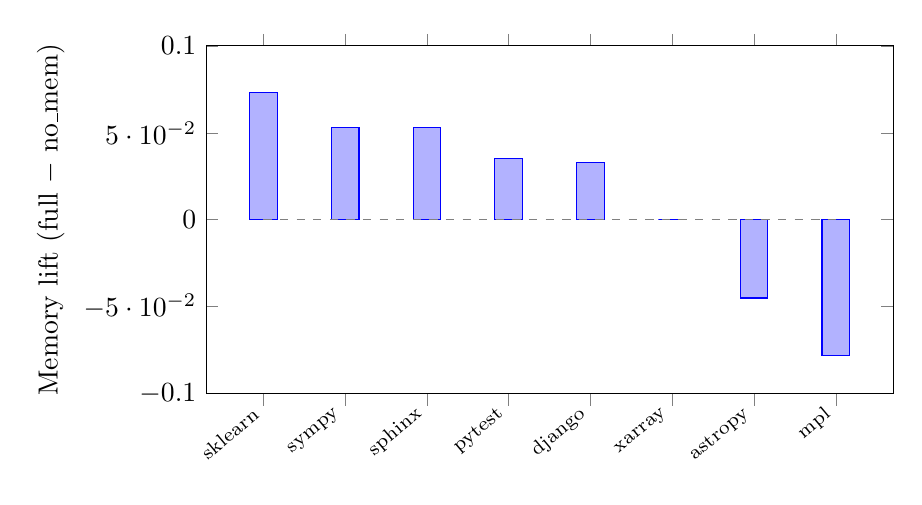
\begin{tikzpicture}\begin{axis}[width=0.85\textwidth,height=6cm,ybar,bar width=10pt,ylabel={Memory lift (full $-$ no\_mem)},
  symbolic x coords={sklearn,sympy,sphinx,pytest,django,xarray,astropy,mpl},xtick=data,
  x tick label style={rotate=40,anchor=east,font=\scriptsize},ymin=-0.10,ymax=0.10]
\addplot coordinates {(sklearn,0.073)(sympy,0.053)(sphinx,0.053)(pytest,0.035)(django,0.033)(xarray,0.000)(astropy,-0.045)(mpl,-0.078)};
\draw[gray,dashed](axis cs:sklearn,0)--(axis cs:mpl,0);
\end{axis}\end{tikzpicture}
\caption{Per-sequence memory lift. Memory helps scikit-learn/sympy/sphinx, hurts
matplotlib/astropy, and does not track structural overlap.}\label{fig:memory-lift}
\end{figure}

\noindent The per-sequence dependency fractions in Table~\ref{tab:memory-lift} are the same
benchmark-structural quantities charted in Figure~\ref{fig:interdependence}; here they serve
as the structural covariate against which the lifts are read.

\subsection{A two-filter account of the bounded benefit}

The lift decomposition and the task-level model below combine into a two-filter explanation
of why the aggregate memory benefit is small even though stored experience is occasionally
decisive. The \emph{first filter} is interdependence: only a minority of tasks
($\approx 0.3$ mean fraction) structurally depend on a predecessor, so by construction memory
cannot help the file-disjoint majority. The \emph{second filter} is utilization: even when a
dependency is present, memory rarely flips the outcome --- the per-sequence lifts are
heterogeneous and frequently negative, and the task-level model (below) finds no policy
effect once difficulty and sequence position are accounted for. The two filters together
shrink a mechanism that is real on specific tasks into an aggregate benefit that the $N=8$
design cannot resolve from zero.

\subsection{Task-level model: position, not policy, governs resolution}

The task-level analysis is a generalized linear mixed model with a binomial/logit link
(Invariant~\#14), fit over all $4{,}914$ task observations with a crossed random effect on
\texttt{task\_id} and \texttt{cls\_consolidation} as the reference policy
(\texttt{glmm\_results.json}; converged). The model isolates the two questions the aggregate
means cannot: whether any policy shifts the per-task odds of resolution once task difficulty
and within-sequence position are controlled, and which covariates actually move the outcome.

No policy coefficient is significant: relative to \texttt{cls\_consolidation},
\texttt{full\_memory} is $+0.116 \pm 0.118$, \texttt{no\_memory} $-0.133 \pm 0.117$,
\texttt{random\_prune} $+0.033 \pm 0.117$, \texttt{recency\_prune} $-0.092 \pm 0.117$, and
\texttt{type\_aware\_decay} $-0.188 \pm 0.117$ --- every one within $2 \times \mathrm{SE}$ of
zero. The policy-null of the sequence-level Wilcoxon (Section~\ref{sec:h1}) therefore holds
at the task level too.

What does move the outcome are the two non-policy covariates. Task difficulty is strongly
negative ($-2.18 \pm 0.065$), as expected, and so is within-sequence position
($-1.49 \pm 0.086$): agent effectiveness \emph{declines across sequence position regardless
of policy}. This is the structural counterpart of the lift result. The agent gets worse as a
sequence progresses --- a trajectory/context-dilution effect --- and crucially, accumulating
memory does \emph{not} rescue it; \texttt{full\_memory}'s task-level odds are statistically
indistinguishable from \texttt{no\_memory}'s. Forgetting is not the cause of late-sequence
decline, and remembering is not its cure.

We report this model on its signs and the null rather than on precise pairwise inference: the
fit is approximate (statsmodels variational estimation; the canonical \texttt{R}/\texttt{lme4}
Laplace fit was not run), and a sensitivity check confirms the direction of the difficulty and
position effects. We do not recompute the untested full-versus-no-memory contrast from the
policy coefficients --- that comparison is the sequence-level Wilcoxon of
Section~\ref{sec:h1}, and reading it off the GLMM coefficients would be test-switching
(Invariant~\#11).

\subsection{Feature analysis: collinearity check passed, helpful/harmful labels deferred}

The pre-registered feature analysis (Invariant~\#13) asks which properties of a retrieved
memory item predict whether it helped or harmed the task it was injected into. The
collinearity prerequisite is satisfied: across $18{,}675$ task--memory pairs the variance
inflation factors are all well below the conventional threshold of $5$ ---
\texttt{semantic\_similarity} $1.42$, \texttt{retrieval\_rank} $1.40$, and
\texttt{memory\_age} $1.02$ --- so the candidate predictors are not redundantly entangled and
a PR-AUC classifier over them would be interpretable.

The classifier itself is deferred. The Tier-1 weak labels available from the run logs are
all-neutral (zero positive instances of the helpful/harmful class), which provides no signal
for a PR-AUC model. Producing the classifier requires Tier-2 manually adjudicated gold
labels, which is downstream work and not a blocker for the headline: the helpful/harmful
prediction would refine \emph{why} a given item helps, but the question of \emph{whether}
memory helps in aggregate is already answered by the lift decomposition and the GLMM above.

\subsection{The anchor-probe sub-study}
\label{sec:a5}

The resolution-rate CL-F1 used throughout this chapter is a proxy; it does not directly
measure continual-learning forgetting or backward retention, and the natural-regime stability
instrument saturates near $1.000$ (Section~\ref{sec:instrument}). To test whether that
saturation reflects genuine robustness or measurement-insensitivity, we ran a separate
construct-validity sub-study --- the A5 anchor probe --- that deliberately constructs cells
where \texttt{full\_memory} retains and retrieves a memory item that a capped pruner has
already evicted. That sub-study is reported as a stand-alone construct-validity analysis and
revisited in the threats-to-validity discussion; it is not part of the H5 task-level model and
does not change the policy-null reported here.

\subsection{Summary}

H5 is, on its surface, a near-null: the aggregate memory benefit is $+1.6$\,pp and
unresolvable from zero. Decomposed, the null is mechanistic rather than empty. Memory helps a
specific minority of sequences, hurts others, and does not track structural overlap; the
benefit it confers is gated by a first filter of interdependence ($\approx 0.3$ of tasks) and
a second filter of utilization (the GLMM policy-null). And the dominant driver of late-sequence
failure --- declining effectiveness with sequence position --- is untouched by how much an
agent remembers. ``Not every task needs memory'' is not a hedge; on this benchmark it is a
measured property, and it is why proactive forgetting is footprint-free on the value axis.
